\externaldocument{../4/chapter_modeling}
\startchapter{Communication Identification Algorithms and Prototype Implementation}
\label{chapter:alo}
In the Modeling Chapter, I elaborate the definition of the communications and the strategy of the communication identification. There are several major step in the identification strategy and some of them are not strange forward. In this chapter, I list developed the algorithms for some steps in the identification strategy. 

\section{Algorithms for Communication Identification in Dual-trace}
All the algorithms list in this section are those key ones in the identification strategy. 

\subsection{Event Locating Algorithm}
The concerned event types in a communication consist of channel open, channel close, send and receive events. Each of these event type would contain one or more functions. The functions list for a communication method is needed as a input of this algorithm. Tables in Section\ref{windows} give the examples of event type list of communication methods. The algorithm is designed for locating events of one communications method. If more than one communication methods are being investigated, this algorithm should be run multiple times, each for a method. Events in the output event list is sorted by time of occurrence, since the search of event is line by line of the assembly instructions.

\begin{algorithm}[H]
\DontPrintSemicolon
\caption{{\bf Event Locating Algorithm} \label{eventLocAlg}}
\KwIn{dual-trace, function list for concerned events}
\KwOut{two event lists for two separative traces in the dual-trace}
$eventLists \leftarrow Map \langle String, List \langle Event\rangle \rangle$;\; 
\For{$trace \in dual$-$trace$}{
   $eventList \leftarrow List \langle Event\rangle$;\; 
   \While{not at end of trace}{
       \For{$f \in functionList$}{
           \If{Is function call of f}{ 
               find function return instruction line;\;          
               $event.inputs \leftarrow$ get input parameters from this instruction line;\;              
               $event.outputs \leftarrow$ get output parameters and return value from the return instruction line;\;
               $event.type \leftarrow f.eventType$;\;
               $eventList.add\left( event \right)$;\;
           }       
        }
    }
    $eventLists.add\left( eventList \right)$;\;
}
\KwRet $eventLists$;\;
\end{algorithm} 

\subsection{Endpoint and Corresponding Streams Identification Algorithm}
The events located in the traces may correspond to different endpoints, the next step is to group them for each endpoints and furthermore group them into streams of the endpoints. The input of this algorithm is one of the event list from the Event Locating Algorithm. So this algorithm should be run separately for both trace in the dual-trace. Since the input event list is sorted by time of occurrence and the channel open events should always happen before other events, it is reasonable to assume the new endpoint can be identified by its first channel open function call. The output of this algorithm is the endpoint list. Each endpoint in this list contains the stream which consist of the sub streams. The concepts of the stream and sub streams are defined in Section\ref{term}. 

\begin{algorithm}[H]
\DontPrintSemicolon
\caption{{\bf Endpoint Indentification Algorithm} \label{endpointIdentAlg}}
\KwIn{event list of a trace}
\KwOut{endpoint list}
$endpoints \leftarrow Map \langle String, List \langle EndPoint\rangle \rangle$;\; 
\For{$event \in eventList$}{
   \If{$event$ is a channel open event}{
      $handle \leftarrow$ get the handle from the function parameter list;\;
      $endpoint \leftarrow endpoints.get\left( handle \right)$;\;
      \If{$endpoint$ is null}{
         $endpoint = New \enspace EndPoint\left( \right)$;\;
         $endpoints.add\left( hanele, endpoint \right)$;\;
      }
      $endpoint.openStream.add\left( event \right)$;\;
   }
   \If{$event$ is a channel send event}{
      $handle \leftarrow$ get the handle from the function parameter list;\;
      $endpoint \leftarrow endpoints.get\left( handle \right)$;\;
      \If{$endpoint$ is not $null$ and $endpoint.complete$ is $False$}{
         $endpoint.sendStream.add\left( event \right)$;\;
      }
   }
   \If{$event$ is a channel receive event}{
      $handle \leftarrow$ get the handle from the function parameter list;\;
      $endpoint \leftarrow endpoints.get\left( handle \right)$;\;
      \If{$endpoint$ is not $null$ and $endpoint.complete$ is $False$}{
         $endpoint.receiveStream.add\left( event \right)$;\;
      }
   }
   \If{$event$ is a channel close event}{
      $handle \leftarrow$ get the handle from the function parameter list;\;
      $endpoint \leftarrow endpoints.get\left( handle \right)$;\;
      \If{$endpoint$ is not null}{
         $endpoint.closeStream.add\left( event \right)$;\;
         $endpoint \leftarrow True$;\;
      }
   }         
}
\KwRet $endpoints$;\;
\end{algorithm} 

\subsection{Channel Identification Algorithm}
The Channel Identification Algorithm aims at identify all the concerned communication channels from the dual-trace. The input of this algorithm is the two endpoint lists for both traces in the dual-trace from the `Endpoint and Corresponding Streams Identification Algorithm'. The output of this algorithm is the channel list. Each channel recognized from the dual-trace contains two endpoints. The channel identification highly depends on the channel opening mechanisms which are different from communication method to communication method. 

In Section\ref{windows}, I elaborate the channel open process for the concerned communication methods. Based on the different process, two algorithms are developed for channel identification, one is for Named Pipe and Message Queue, while the other is for TCP and UDP. For the Named pipe and MSMQ only one channel open function is being call for each endpoint. And the identification is basically done by matching the endpoints with their channel identifier. The channel Identifier for Named pipe is the file name while for MSMQ is the queue format name as input in the channel open functions. But for TCP and UDP multiple functions are collaborating to form the final communication channel. Remote and local addresses and ports of each endpoint are used to identify the channel. 

\subsubsection{For Named pipe and Message Queue}
This algorithm will find out all the possible channels regardless some of them might be false positive. For example, the server is connected by two clients with the file as the channel. In the server trace, there are two endpoints found. In each client trace, there is one endpoint found. In the channel identification algorithm for the dual-trace of server and client1, there will be two possible identified channels, one is the real used one for server and client1 while the other is the false positive one actually is for server and client2. The endpoint in client1's trace will be matched by two endpoints in the server's trace. In this step in the communication identification, there is no way to district these two channels. One solution is to further check the sent and receive data to verify if the channel is real. However if the data be transmitted in both located channel are identical, there is still no way to exclude the false positive ones unless more information such as timing of the captured traces is provided.

And other example of Named pipe is the same file is reused for multiple times by the endpoint pairs, without further information it's hard to align endpoint matches.

These errors are also applicable for Message Queue Communications.

\begin{algorithm}[H]
\DontPrintSemicolon
\caption{{\bf Channel Indentification Algorithm for Named pipe and Message Queue} \label{channelAlg1}}
\KwIn{two endpoint lists of the dual-trace}
\KwOut{channel list}
$channels \leftarrow Map \langle String, List \langle Channel \rangle \rangle$;\; 
\For{$endpoint \in endpointList1$}{
   $openEvent1 \leftarrow$ get the event from $endpoint.openStream$, which should only contain one event. 
   $channelId1 \leftarrow$ get the channel identifier from $openEvent1.inputs$;\;
   \For{$endpoint2 \in endpointList2$}{
      $openEvent2 \leftarrow$ get the event from $endpoint2.openStream$, which should only contain one event.
      $channelId2 \leftarrow$ get the channel identifier from $openEvent2.inputs$;\;
    \If{$channelId1 == channelId2$}{
       $channel = New \enspace Channel()$;\;
       $channels.add\left( channel \right)$;\;
    }
   }
}
\KwRet $channels$;\;
\end{algorithm} 

\subsubsection{For TCP and UDP}
This false positive situation will be a lot better for TCP and UDP transmissions due to the rarely two applications on hosts share the same address and port. So we can assume that the problem of mismatching the endpoints from different host would not happen. However, we can not avoid the address and port being reused by multiple endpoints in the same application. So the false positive error would still happen. The data verification algorithm in later section can help to reduce the error and what is good is that as long as we can find one district channel data from the multiple matching set we can align all of the endpoints from that set properly and exclude the false positive ones. The scenarios of channel(or address and port) reusing are list in Figure. The first scenario represents the transmitted data in all reused endpoint set are identical, while the second one contains district transmitted data in at least one endpoint pair.

\begin{figure}[H]
\centerline{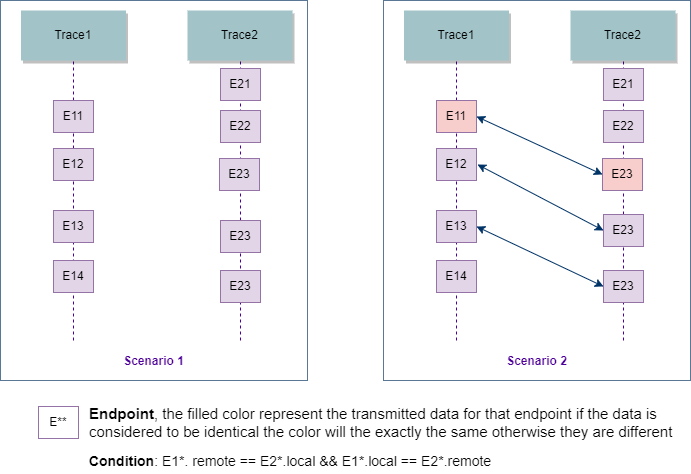
\includegraphics[scale=0.55]{Figures/channelreusetcpudp}}
 \caption{Channel Reuse Scenarios}
\label{communicationhappen}
\end{figure}

\begin{algorithm}[H]
\DontPrintSemicolon
\caption{{\bf Channel Indentification Algorithm for TCP and UDP} \label{channelAlg1}}
\KwIn{two endpoint lists of the dual-trace}
\KwOut{channel list}
$channels \leftarrow Map \langle String, List \langle Channel \rangle \rangle$;\; 
\For{$endpoint \in endpointList1$}{
   $openEvent1 \leftarrow$ get the event from $endpoint.openStream$, which should only contain one event. 
   $channelId1 \leftarrow$ get the channel identifier from $openEvent1.inputs$;\;
   \For{$endpoint2 \in endpointList2$}{
      $openEvent2 \leftarrow$ get the event from $endpoint2.openStream$, which should only contain one event.
      $channelId2 \leftarrow$ get the channel identifier from $openEvent2.inputs$;\;
    \If{$channelId1 == channelId2$}{
       $channel = New \enspace Channel()$;\;
       $channels.add\left( channel \right)$;\;
    }
   }
}
\KwRet $channels$;\;
\end{algorithm}

\subsection{Transported Stream Data Verification}

\subsection{Transported Event Data Verification}

\subsection{Data Structure for Identified Communications}

\section{Communication Identification Feature Prototype}
